\documentclass{article}

\usepackage[usenames, dvipsnames]{color}
%set up line color that represents each phase of study
\definecolor{qualitative}{rgb}{0.85,0.85,0.85}
\definecolor{listing}{rgb}{0.75,0.75,0.75}
\definecolor{base}{rgb}{0.6,0.6,0.6}
\definecolor{treat}{rgb}{0.45,0.45,0.45}
\definecolor{end1}{rgb}{0.3,0.3,0.3}
\definecolor{end2}{rgb}{0,0,0}


\usepackage{graphics}
\usepackage{tikz}
\usepackage{color,xcolor}
\usetikzlibrary{snakes}
\usepackage[document]{ragged2e}

\begin{document}


	\centering
	{FIGURE 1: STUDY TIMELINE} \\ [1.5ex]
		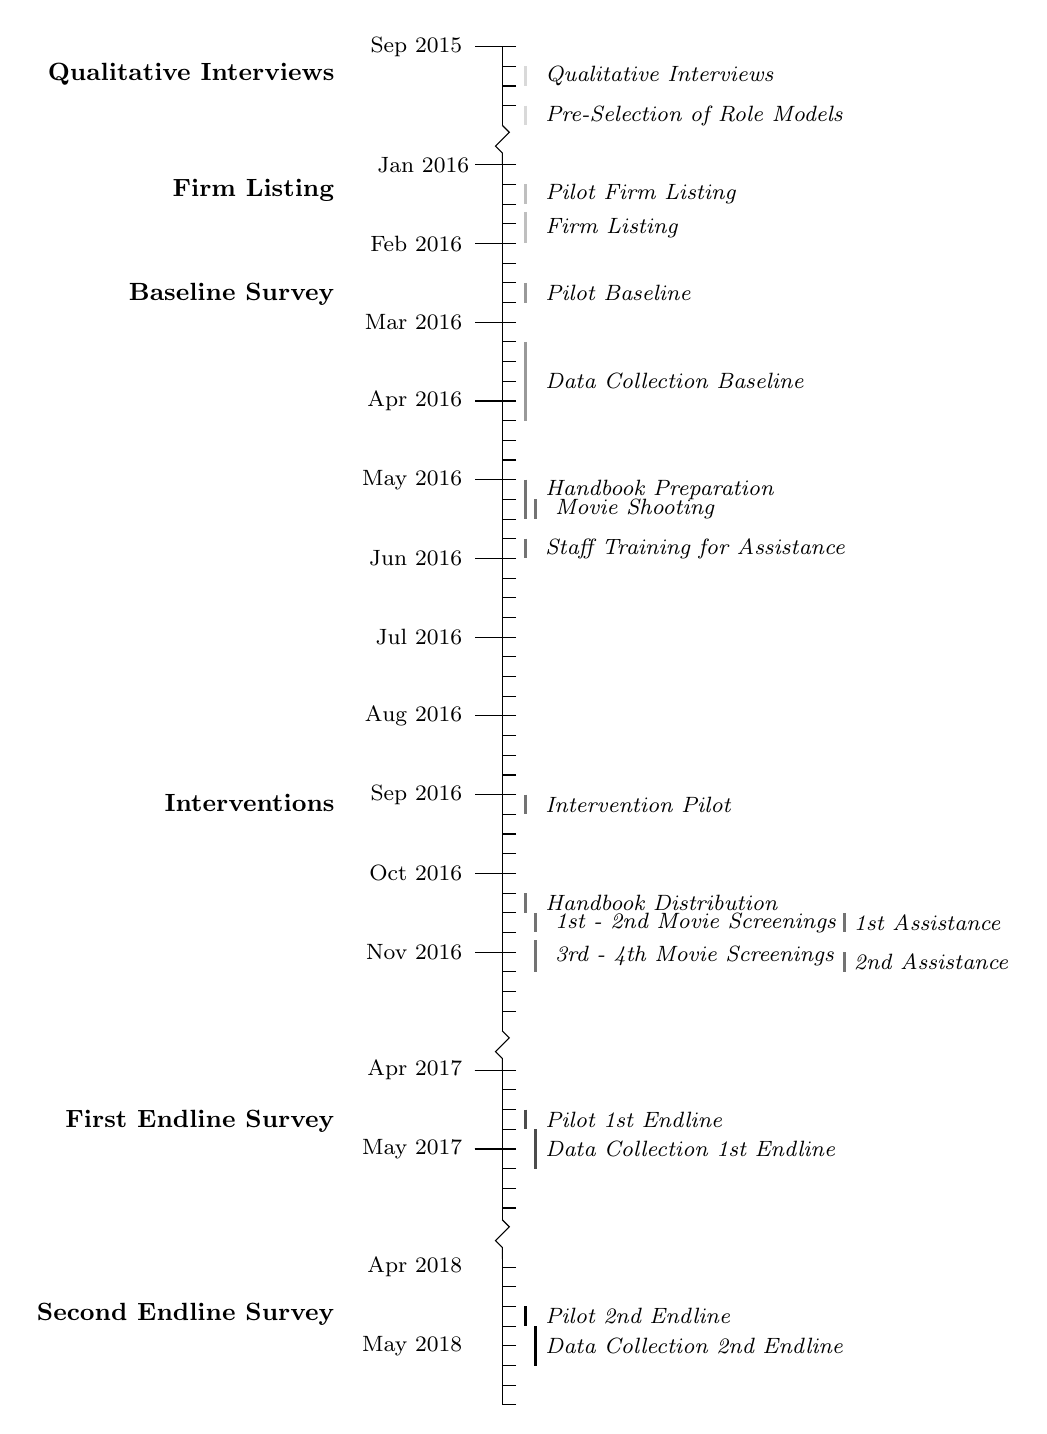
\begin{tikzpicture}[node distance=5mm]
		%draw vertical line
		% Pre-baseline
		\draw			(0,-1) -- (0,0);
		\draw[snake] 	(0,-1) -- (0,-1.5);	
		% Baseline
		\draw			(0,-1.5) -- (0,-5);
		% Interventions
		\draw			(0,-5) -- (0,-12.5);
		% First endline
		\draw[snake]	(0,-12.5) -- (0,-13);
		\draw			(0,-13) -- (0,-14.90);
		% Second endline
		\draw[snake]	(0,-14.90) -- (0,-15.40);
		\draw			(0,-15.40) -- (0,-17.25);	

		% Draw horizontal line for major events
		\foreach	\y in {-1.5,-2.5,-5.5}
		\draw	(0,\y) -- (5pt, \y);
		
		% Qualitative interviews
		\draw(-0.25,-0.35)node{}node[left=50pt]{\small \textbf {Qualitative Interviews}};
		\foreach \y in {0}
		\draw (0,\y) -- (-10pt,\y);
			\draw(0,0)node{}node[left=11pt]{\footnotesize {Sep 2015}};
				\foreach \y in {0,-0.25,-0.5,-0.75}
				\draw (5pt, \y) -- (0,\y);
				\draw(0,-0.375)node{}node[right=12pt]{\footnotesize \textit {Qualitative Interviews}};
					\draw[line width=0.35mm,qualitative](8.5pt,-0.25)--(8.5pt,-0.5); %draw line for qualitative and role model interviews
				\draw(0,-0.875)node{}node[right=12pt]{\footnotesize \textit {Pre-Selection of Role Models}};
					\draw[line width=0.35mm,qualitative](8.5pt,-0.75)--(8.5pt,-1); %draw line for qualitative and role model interviews

		% Listing
		\draw(-0.25,-1.83)node{}node[left=50pt]{\small \textbf {Firm Listing}};
		\foreach \y in {-1.5}
		\draw (0,\y) -- (-10pt,\y);
			\draw(0,-1.5)node{}node[left=8.5pt]{\raggedleft \footnotesize {Jan 2016}};
				\foreach \y in {-1.5,-1.75,-2,-2.25}
				\draw (5pt, \y) -- (0,\y);
				\draw(0,-1.875)node{}node[right=12pt]{\footnotesize \textit {Pilot Firm Listing}};
					\draw[line width=0.35mm, listing](8.5pt,-1.75)--(8.5pt,-2); %draw line for firm listing period
				\draw(0,-2.3)node{}node[right=12pt]{\footnotesize \textit {Firm Listing}};
					\draw[line width=0.35mm, listing](8.5pt,-2.1)--(8.5pt,-2.5); %draw line for firm listing period
		
		% Baseline survey
		\draw(-0.25,-3.15)node{}node[left=50pt]{\small \textbf {Baseline Survey}};
		\foreach \y in {-2.5,-3.5,-4.5}
		\draw (0,\y) -- (-10pt,\y);
			\draw(0,-2.5)node{}node[left=11pt]{\footnotesize {Feb 2016}};
				\foreach \y in {-2.5,-2.75,-3,-3.25}
				\draw (5pt, \y) -- (0,\y);
				\draw(0,-3.125)node{}node[right=12pt]{\footnotesize \textit {Pilot Baseline}};
					\draw[line width = 0.35mm, base](8.5pt,-3)--(8.5pt,-3.25); %draw line for baseline pilot period
			\draw(0,-3.5)node{}node[left=11pt]{\footnotesize {Mar 2016}};
				\foreach \y in {-3.5,-3.75,-4,-4.25}
				\draw (5pt, \y) -- (0,\y);
				\draw(0,-4.25)node{}node[right=12pt]{\footnotesize \textit {Data Collection Baseline}};
					\draw[line width = 0.35mm, base](8.5pt,-3.75)--(8.5pt,-4.75); %draw line for baseline data collection period
			\draw(0,-4.5)node{}node[left=11pt]{\footnotesize {Apr 2016}};
				\foreach \y in {-4.5,-4.75,-5,-5.25}
				\draw (5pt, \y) -- (0,\y);
			
		% Interventions
		\draw(-.25,-9.6)node{}node[left=50pt]{\small \textbf {Interventions}};
		\foreach \y in {-5.5,-6.5,-7.5,-8.5,-9.5,-10.5,-11.5}
		\draw (0,\y) -- (-10pt,\y);
		\draw(0,-5.5)node{}node[left=11pt]{\footnotesize {May 2016}};
				\foreach \y in {-5.5,-5.75,-6,-6.25}
				\draw (5pt, \y) -- (0,\y);
				%special rule for handbook preparation and shooting layout, where it's not put in the middle of the line but in the middle of week's space (\y)
				%for example handbook preparation, where it's put at "-5.625", resulting from diff between weeks (\y, -((0.25/2)+5.5)
				\draw(0,-5.625)node{}node[right=12pt]{\footnotesize \textit {Handbook Preparation}};
					\draw[line width = 0.35mm,treat](8.5pt,-5.5)--(8.5pt,-6); %draw line for handbook preparation
				\draw(0,-5.875)node{}node[right=15.5pt]{\footnotesize \textit {Movie Shooting}};
					\draw[line width = 0.35mm, treat](12pt,-5.75)--(12pt,-6); %draw line for shooting of the movie
				\draw(0,-6.375)node{}node[right=12pt]{\footnotesize \textit {Staff Training for Assistance}};
					\draw[line width = 0.35mm, treat](8.5pt,-6.25)--(8.5pt,-6.5); %draw line for staff training
		\draw(0,-6.5)node{}node[left=11pt]{\footnotesize {Jun 2016}};
				\foreach \y in {-6.5,-6.75,-7,-7.25}
				\draw (5pt, \y) -- (0,\y);
		\draw(0,-7.5)node{}node[left=11pt]{\footnotesize {Jul 2016}};
				\foreach \y in {-7.5,-7.75,-8,-8.25}
				\draw (5pt, \y) -- (0,\y);
		\draw(0,-8.5)node{}node[left=11pt]{\footnotesize {Aug 2016}};
				\foreach \y in {-8.5,-8.75,-9,-9.25}
				\draw (5pt, \y) -- (0,\y);
		\draw(0,-9.5)node{}node[left=11pt]{\footnotesize {Sep 2016}};
				\foreach \y in {-9.5,-9.75,-10,-10.25}
				\draw (5pt, \y) -- (0,\y);
				\draw(0,-9.625)node{}node[right=12pt]{\footnotesize \textit {Intervention Pilot}};
					\draw[line width=0.35mm, treat](8.5pt,-9.5) -- (8.5pt,-9.75); %draw line for intervention pilot
		\draw(0,-10.5)node{}node[left=11pt]{\footnotesize {Oct 2016}};
				\foreach \y in {-10.5,-10.75,-11,-11.25}
				\draw (5pt, \y) -- (0,\y);
				\draw(0,-10.875)node{}node[right=12pt]{\footnotesize \textit {Handbook Distribution}};
					\draw[line width=0.35mm, treat](8.5pt,-10.75) -- (8.5pt,-11); %draw line for handbook distribution period
				\draw(0,-11.125)node{}node[right=15.5pt]{\footnotesize \textit {1st - 2nd Movie Screenings}};
					\draw[line width=0.35mm, treat](12pt,-11)--(12pt,-11.25); %draw line for 1st - 2nd movie screenings period (obligatory for all kelurahans. explain in notes)
				\draw(0,-11.125)node{}node[right=123.5pt]{\footnotesize \textit {1st Assistance}};
					\draw[line width = 0.35mm, treat](123.5pt,-11)--(123.5pt,-11.25); %draw line for 1st assistance period
		\draw(0,-11.5)node{}node[left=11pt]{\footnotesize {Nov 2016}};
				\foreach \y in {-11.5,-11.75,-12,-12.25}
				\draw (5pt, \y) -- (0,\y);
				\draw(0,-11.55)node{}node[right=15.5pt]{\footnotesize \textit {3rd - 4th Movie Screenings}};
					\draw[line width=0.35mm, treat](12pt,-11.35)--(12pt,-11.75); %draw line for 3rd - 4th movie screenings period (only for kelurahans with low attendance. explain in notes)
				\draw(0,-11.625)node{}node[right=123.5pt]{\footnotesize \textit {2nd Assistance}};
					\draw[line width = 0.35mm, treat](123.5pt,-11.5)--(123.5pt,-11.75); %draw line for 2nd assistance period

	% endline
		\draw(-0.25,-13.65)node{}node[left=50pt]{\small \textbf {First Endline Survey}};
			\foreach \y in {-13,-14}
			\draw (-10pt,\y) -- (0,\y);
		\draw(0,-13)node{}node[left=11pt]{\footnotesize {Apr 2017}};
			\foreach \y in {-13,-13.25,-13.5,-13.75}
			\draw (5pt,\y) -- (0,\y);
				\draw(0,-13.625)node{}node[right=12pt]{\footnotesize \textit {Pilot 1st Endline}};
					\draw[line width=0.35mm, end1](8.5pt,-13.5)--(8.5pt,-13.75); %draw line for endline data collection period
				\draw(0,-14)node{}node[right=12pt]{\footnotesize \textit {Data Collection 1st Endline}};
					\draw[line width=0.35mm, end1](12pt,-13.75)--(12pt,-14.25); %draw line for endline data collection period
		\draw(0,-14)node{}node[left=11pt]{\footnotesize {May 2017}};
			\foreach \y in {-14,-14.25,-14.5,-14.75}
			\draw (5pt,\y) -- (0,\y);
			
		% endline 2
		\draw(-.25,-16.1)node{}node[left=50pt]{\small \textbf {Second Endline Survey}};
			\foreach \y in {-13,-14}
			\draw (-10pt,\y) -- (0,\y);
		\draw(0,-15.5)node{}node[left=11pt]{\footnotesize {Apr 2018}};
			\foreach \y in {-15.5,-15.75,-16.0,-16.25}
			\draw (5pt,\y) -- (0,\y);
				\draw(0,-16.125)node{}node[right=12pt]{\footnotesize \textit {Pilot 2nd Endline}};
					\draw[line width=0.35mm, end2](8.5pt,-16.0)--(8.5pt,-16.25); %draw line for endline data collection period
				\draw(0,-16.5)node{}node[right=12pt]{\footnotesize \textit {Data Collection 2nd Endline}};
					\draw[line width=0.35mm, end2](12pt,-16.25)--(12pt,-16.75); %draw line for endline data collection period
		\draw(0,-16.5)node{}node[left=11pt]{\footnotesize {May 2018}};
			\foreach \y in {-16.50,-16.75,-17.0,-17.25}
			\draw (5pt,\y) -- (0,\y);

		\end{tikzpicture}

\end{document} 